% !TEX program = arara-rc
% !TEX encoding = utf8
% !TEX spellcheck = en_GB
%:!arara settings
% arara: lualatex: { shell: true , synctex: true }
% !arara: lualatex: { shell: true , synctex: true }
%%: Start Header
\makeatletter
\RequirePackage{ifluatex}
\ifluatex
 \else
   \PackageError{xframed}{
    ^^J\space\space * This file requires LuaTeX.       
    ^^J\space\space * You  must change your typesetting engine                
  }
  \expandafter\endinput
\fi
\makeatother
\setcounter{errorcontextlines}{999}
\documentclass[openany,12pt,tocdepth=3,showframe]{ltx-md}
\RequirePackage{minted}
\usemintedstyle{friendly}
\fvset{xleftmargin=1cm,xrightmargin=1cm}
\renewcommand*{\dictumwidth}{.5\textwidth}
\setcounter{secnumdepth}{3}

\ExplSyntaxOn
\keys_define:nn {ltxexample}
 {
  caption  .tl_set:N = \l_mdxex_caption_tl,
  label    .tl_set:N = \l_mdxex_label_tl,
  minted   .tl_set:N = \l_mdxex_minted_tl,
  minted   .initial:n = {linenos=true} ,
  language .tl_set:N = \l_mdxex_language_tl,
  language .initial:n = latex,
 }

\NewDocumentEnvironment {ltxexample} { O {} }
 {\group_begin:
  \keys_set:nn { ltxexample }
   {
    #1
   }
  \tl_set:Nx \l__mdxex_temp_tl
   {
    \exp_not:N \VerbatimEnvironment
    \tl_if_empty:NTF \l_mdxex_caption_tl
     {
      \scan_stop:
     }
     {
      \exp_not:N \captionof { lstlisting }{ \exp_not:V \l_mdxex_caption_tl }
      \tl_if_empty:NF \l_mdxex_label_tl
       { \exp_not:N \label { \l_mdxex_label_tl } }
     }
    \exp_not:n { \begin{minted} } [ \l_mdxex_minted_tl ] { \l_mdxex_language_tl }
   }
  \l__mdxex_temp_tl
 }
 {\end{minted}\group_end:}
\RenewDocumentCommand\DeleteFile{m}{}
\ExplSyntaxOff
\NewDocumentCommand \Github {} {Github\faGithub\xspace }
\usepackage{xframed}
\begin{document}
\title{The \Pack{xframed} package}
\subtitle{This is an alpha-version}
\author{Marco Daniel}
\date{\today}
\notes{As shown in the subtitle this is an alpha version. Use this package on your own
risk.\\[.5cm]
I know my English is really poor and the quality of the documentation suffers on it. 
So I am really happy about any improvments.\\[1cm]

As long as the package has the version alpha I am not deprecated to change names
of options. My aim is to use as many intuitive options as possible. 
}
\maketitle
\clearpage
\pdfbookmark[1]{\contentsname}{tocbook}
\tableofcontents
\addchap{Preface}
\addsec{Introduction}\label{sec:intro}
I am interested in \LaTeX\ and specially in \LaTeX3. With this package I want
to improve my skills using this great language. However I am a beginner and
so the package has only an \textit{alpha} version. If you use this package
be aware of this situation. I am sure the great guys at
\faArrowRight\href{http://tex.stackexchange.com/}{TeX.SX} will help me to improve this package.


\addsec{Bug reports}\label{sec:bug-reports}
Bug reports can be done at
\href{https://github.com/marcodaniel/xframed/issues}{xframed at \Github}. If you have no
account at \Github you can drop me an e-mail
\href{mailto:marco.daniel@mada-nada.de}{\faEnvelope marco.daniel@mada-nada.de}

\addsec{Installation}
As long as the package isn't available at CTAN you must install (if you dare it)
manual. Therefor you can clone the repository in your local texmf tree. I provided
the correct folder structure at \Github to simplify the installation.

\setchapterpreamble[o]{\dictum[]{%
If you are only interested in the usage of the package you can
skip this chapter. All options are explain in \autoref{chap:usage}}}
\chapter{Idea behind \texorpdfstring{\Pack{xframed}}{xframed}}\label{chap:idea}

The idea is very simple. Draw a frame around given material. During my study 
I wanted a package which can be break across pages and put a frame around this.
The package \Pack{framed}\footnote{Package \Pack{framed} by Don­ald Arse­neau, 
see \href{http://www.ctan.org/pkg/framed}{CTAN: framed}} didn't require my needs.
So I started to write my own package. The result can be found at CTAN, too. It's the
package \Pack{mdframed}\footnote{Package \Pack{mdframed} by Marco Daniel, 
see \href{http://www.ctan.org/pkg/mdframed}{CTAN: mdframed}}.

After passing my study I started to improve the package \Pack{mdframed}. In 2011 
I registered at \href{http://tex.stackexchange.com/}{TeX.SX}  and learned something
about the new language \Pack{expl3}\footnote{see: 
\href{http://latex-project.org/latex3.html}{http://latex-project.org/latex3.html}}. 
I was so fascinated about the great work of the \LaTeX3 core team that I started 
my first steps with simple function. After a while I wanted to provide my
own \Pack{expl3}-package. Now here it is.

I know most users love examples. So I am trying to provide a lot. All
frames in this documentation are done by \Env{xframed}. So I hope
you will have some inspiration.

\vfill
By the way. The compiliation is of this document is done with the
typesetting enginge \LuaLaTeX. To simplify my compilation steps
I am using \Pack{arara}\footnote{Tool \Pack{arara} by Paulo Cereda, 
see \href{http://www.ctan.org/pkg/arara}{CTAN: arara}}.

\vfill
Now it's time to introduce the package.



\chapter{Usage}\label{chap:usage}
The following sections descripe the options of the package and the provided 
environments. The basic environment is equal to the package name \Env{xframed}.

\section{Loading the package}
Before you can use the package, you must load it in your preamble. As usual the 
package is loaded by \Cmd{usepackage}. The following listings shows it.
\begin{ltxexample}[caption=Loading the package,label=loading]
 % Preamble
 \usepackage{xframed}
\end{ltxexample}
If you have done this you can use the basic environment \Env{xframed}.

\ExplEnv{xframed}
The environment has one optional argument where you can specify options
which are only used for this frame. The following listings demonstrates the usage.
\begin{ltxexample}[caption=Loading the package,label=loading]
 % document body
 \begin{xframed}[option-list]
   The contents of the frame
 \end{xframed}
\end{ltxexample}

\section{Specifying the options}
Before you setup any options you must understand hot the frame is drawn.
The default method is by using \Pack{TikZ}\footnote{Package \Pack{TikZ} by 
Till Tantau \& friends, see \href{http://www.ctan.org/pkg/pgf}{CTAN: TikZ}}. 
\Pack{TikZ} allows a very user friendly way to setup high quality graphics. 
Therefor all elements are specified by \Pack{TikZ} options. The basic command
to manipulate these elements is \Cmd{xframedsetuptikz}. The usage is explained
in \autoref{se:tikzsetup}.  All other options can be set by \Cmd{xframedsetup}. 
Both command can be used in the preamble or inside the document body. If
you enclose these commands inside a group the settings will be local, too.
 
\ExplCmd{xframedsetuptikz\MArgs}
The command has one mandatory argument. The mandatory argument accepts only
defined options which are explaind in \autoref{se:tikzsetup}

All other options can be setup by the command \Cmd{xframedsetup}.
\ExplCmd{xframedsetup\MArgs}
This command has one mandatory argument. All allowed options are explained
in \autoref{chap:options}. 

Before we start with options we need to understand the provided elements of the frame. 

\section{Elements of the frame drawn by \texorpdfstring{\Pack{xframed}}{xframed}}
It should be clear the a frame has some rules around. So we can check mark the first
relevant point.The next point of the agende is the main body, the title and the foot. These
three elements are very important to understand the behaviour. The simple picture below
should show the elements and the provided names inside the package.

\begin{center}
\captionof{figure}{Base elements of \texorpdfstring{\Pack{xframed}}{xframed}}\label{fig:baseelements}
\begin{tikzpicture}[outer sep=0pt]
 \node[draw,rectangle,minimum width=8cm, minimum height=2cm,font=\bfseries] (main) {Body of the frame~\faArrowRight~\texttt{main}};
 \node[draw,rectangle,minimum width=8cm, minimum height=1cm,font=\bfseries,anchor=south] at (main.north) {Title of the frame~\faArrowRight~\texttt{first-title}};
 \node[draw,rectangle,minimum width=8cm, minimum height=1cm,font=\bfseries,anchor=north] at (main.south) {Foot of the frame~\faArrowRight~\texttt{last-foot}};
\end{tikzpicture}
\end{center}
I know the picture looks very poor at the beginning but we want to concentrate on the
main issue. It descripes the three base elements of the frame drawn by \Env{xframed}.

\vspace*{\baselineskip}
Now let's start with all options. Be aware the list ist long. 

\setchapterpreamble[o]{\dictum[]{%
The quality of the frame depends on your skill to use
the options.}}

\chapter{Package options}\label{chap:options}
Every user has his/her own wishes. It's very difficult to implement an evironment 
which meets all requirements. I hope with the following options you can setup your 
requirements as best as I was able to implement. As described in \autoref{chap:idea}
the package uses \Pack{expl3} in the background. So I can provide more intuitive names.
During the explanation I refer to the environment \Env{framed}. However this is only
symbolic. The options are also working for other derivations. 

\section{Outside the frame}
Drawing a frame requires some modifcations around. So you want to setup the margins
or the skips above or below the frame. Related to the meaning of the keys, all keys 
requiers a length or skip dimension. That mean that the length variables defined as
\texttt{dim} have a fixed length, whereas \texttt{skip} length can have a rupper (stretch/shrink) component. 

\ExplOpt{skip}
This is the length represented the space before and after the environment \Env{xframed}.  
This options is a meta key and sets the \Opt{skip-below} and \Opt{skip-above} to the given skip length. 
\ExplOpt[10pt]{skip-above}
As described at \Opt{skip} this skip length specify the space above the frame.
\ExplOpt[10pt]{skip-below}
Related to the other options here you can setup the space after the environment.


\ExplOpt{margin}
Normally the frame \Env{xframed} is drawn about the complete text width. However this isn't
often very common. This keys accept a dimension length which specify the left and the right margin.
You can also use negativ values. In this case the frame is drawn inside the margin of the page.
\ExplOpt[0\,pt]{left-margin}
Here you can setup the left margin separat. 
\ExplOpt[0\,pt]{right-margin}
And here the right margin. 

\vspace*{\baselineskip}
This finished the \emph{outside} part for the moment. The package provides also some hooks
which will can be used as an option. This isn't really a low level issue so these
options are desribed in \autoref{sec:hook}. 

\vspace*{\baselineskip}
Before I will descripe the options related to there base element as shown in \autoref{fig:baseelements}, 
I will start with the rules around the frame.

\section{Rules around the frame}\label{sec:lines}
A normal frame has four sides. The frame of \Env{xframed} isn't an exception. Of course
you can manipulate as possible to get a triangle or a star.

\ExplOpt{line-width}
The first option in this section specify the width of all four lines around the material of \Env{xframed}.
This implices the title and the foot of the frame. If you want to setupt the rule width of the elements
separate you can do this by the following options.
\ExplOpt[0.8\,pt]{line-width-left}
Specifies the width of the left line.
\ExplOpt[0.8\,pt]{line-width-right}
Specifies the width of the right line.
\ExplOpt[0.8\,pt]{line-width-top}
Specifies the width of the top line.
\ExplOpt[0.8\,pt]{line-width-bottom}
Specifies the width of the bottom line.

\minisec{Example}
I think it's time for a small example. Suppose you want that all lines has a width of
2\,pt expect the top line which shall have a width of 4pt. This can be achived by
\begin{ltxexample}[caption=Loading the package,label=loading]
 \begin{xframed}[line-width=2pt,line-width-top=4pt]
   The contents of the frame
 \end{xframed}
\end{ltxexample}
As a small revision we can achive the same effect with \Cmd{xframedsetup}, 
whereby the settings are used for the the environemnts \Env{xframed} to follow.
\begin{ltxexample}[caption=Loading the package,label=loading]
 \xframedsetup[line-width=2pt,line-width-top=4pt]
 \begin{xframed}
   The contents of the frame
 \end{xframed}
\end{ltxexample}

\begin{xframed}[line-width=2pt,line-width-top=4pt,left-margin=0pt]
   The contents of the frame
\end{xframed}

\section{Main body of the frame}\label{sec:element-main}

\section{Title of the frame}\label{sec:element-firsttitle}

\section{Foot of the frame}\label{sec:element-lastfoot}



\section{Tikz elements of  \texorpdfstring{\Pack{xframed}}{xframed}}


\section{Hooks}\label{sec:hook}

\label{se:tikzsetup}

\chapter{Developer Info}\label{chap:developer-info}


\chapter{Appendix}\label{chap:appendix}
\section{Thanks}

\section{Bugs}
\end{document}
